%%=================================================================
%% UFAC-modelo-TCC.tex (UTF-8 format), v1.0
%%
%% Adaptação do Modelo de Trabalho de Conclusão de Curso (TCC) do
%% curso de Bacharelado em Sistemas de Informação da Universidade
%% Federal do Acre em LaTeX utilizando o pacote abnTeX2
%% (http://abnTeX2.googlecode.com).
%%=================================================================

\documentclass[
    % -- opções da classe memoir --
    12pt,               % Tamanho da fonte
    openright,          % Capítulos começam em pág. ímpar (insere página vazia caso preciso)
    oneside,            % Impressão apenas no anverso. Oposto a opção "twoside"
    a4paper,            % Tamanho do papel
    % -- opções do pacote abntex2 --
    chapter=TITLE,      % Títulos de capítulos, de elementos pré-textuais e pós-textuais em maiúsculas
    sumario=tradicional,% Sumário padrão memoir. Oposto a opção "abnt-6027-2012"
    % -- opções do pacote babel --
    english,            % Idioma adicional para hifenização
    brazilian,          % Idioma principal do documento (Corrigido para evitar o warning)
 ]{abntex2}


%% CONFIGURAÇÕES DE PACOTES

% Pacotes básicos
\usepackage{lmodern}            % Usa a fonte Latin Modern
\usepackage[T1]{fontenc}        % Seleção de códigos de fonte de saída
\usepackage[utf8]{inputenc}     % Codificação do documento (conversão automática dos acentos)
\usepackage{indentfirst}        % Indenta o primeiro parágrafo de cada seção
\usepackage{graphicx}           % Inclusão de gráficos e figuras
\graphicspath{{figures/}}       % Diretório padrão para imagens do projeto
\usepackage{booktabs}           % \toprule, \midrule e \bottomrule para tabelas
\usepackage{pgfgantt}           % para usar o gráfico de gant

% Sistema (Autor, data) com títulos das referências em negrito e termo latino "et al." escrito em itálico
\usepackage[alf,abnt-emphasize=bf, abnt-etal-text=it]{abntex2cite}
\bibliographystyle{abntex2-alf.bst}

% Títulos em fonte Times
\usepackage{mathptmx}
\renewcommand{\ABNTEXchapterfont}{\rmfamily\bfseries}
\renewcommand{\ABNTEXchapterfontsize}{\LARGE}
\renewcommand{\ABNTEXsectionfont}{\rmfamily\bfseries}
\renewcommand{\ABNTEXsectionfontsize}{\Large}
\renewcommand{\ABNTEXsubsectionfont}{\rmfamily\bfseries}
\renewcommand{\ABNTEXsubsectionfontsize}{\small}
\renewcommand{\ABNTEXsubsubsectionfont}{\rmfamily\bfseries}
\renewcommand{\ABNTEXsubsubsectionfontsize}{\small}
\usepackage{tikz}
\usetikzlibrary{arrows.meta, positioning, shapes}
% Leitura de figuras .eps, compilação para PDF
\usepackage[outdir=./]{epstopdf}
\usepackage{epsfig}

%\usepackage{abntex2-UFAC}       % Personalização de ESTILO para a Universidade Federal do Acre

% Pacotes adicionais
\usepackage{pgfplots, pgfplotstable}
\pgfplotsset{compat=1.15}

\usepackage{xcolor}             % Controle das cores
\usepackage{microtype}          % Para aprimoramento do arranjo visual do texto na ferramenta OVERLEAF
\usepackage{amsmath}            % Pacote para controle de equações matemáticas
\usepackage{float}
\usepackage{enumitem}
\usepackage{pgf-pie}

\newfloat{quadro}{htbp}{loq}
\floatname{quadro}{Quadro}
\newcommand{\listofquadrosname}{Lista de quadros}
\newcommand{\listofquadros}{\listof{quadro}{\listofquadrosname}}

% Termos latinos para serem escritos em itálico
\renewcommand{\apudname}{\textit{apud}}
\renewcommand{\passimname}{\textit{passim}}
\renewcommand{\Idemname}{\textit{Id.}}
\renewcommand{\Ibidemname}{\textit{Ibid.}}
\renewcommand{\opcitname}{\textit{op.\ cit.}}
\renewcommand{\loccitname}{\textit{loc.\ cit.}}
\renewcommand{\cfcitename}{\textit{Cf.}}
\renewcommand{\etseqname}{\textit{et seq.}}
% ---

%% Informações de dados para CAPA e FOLHA DE ROSTO
\titulo{Ciência de Dados Aplicada Na Detecção de Anomalias em Portais de Transparências: Um Estudo de Caso do Governo do Estado do Acre}

\autor{Guilherme de Jesus Carvalho}

\local{Rio Branco}

\data{\the\year}

\orientador{Prof. Dra. Laura Costa Sarkis}
\coorientador{Prof. Dra. Lorena Caceres Tomaya}

% AQUI ESTÁ O TRUQUE PARA FORÇAR A SUA IMAGEM NA CAPA
\instituicao{Universidade Federal do Acre}

\makeatletter
\renewcommand{\imprimircapa}{%
  \begin{capa}%
    \center
    
\includegraphics[width=2.5cm]{brasaoufac.png}\par
    \vspace{0.5cm}
    {\ABNTEXchapterfont\large\imprimirinstituicao}

    \vspace{2cm}
    {\ABNTEXchapterfont\large\imprimirautor}

    \vspace*{\fill}
    \begin{center}
      \ABNTEXchapterfont\bfseries\Large\imprimirtitulo
    \end{center}
    \vspace*{\fill}

    {\large\imprimirlocal}
    \par
    {\large\imprimirdata}

    \vspace*{1cm}
  \end{capa}%
}
\makeatother

%% Configurações de aparência do PDF final
\makeatletter
\hypersetup{
    pdftitle={\@title},
    pdfauthor={\@author},
    pdfsubject={\imprimirpreambulo},
    pdfcreator={LaTeX with abnTeX2},
    colorlinks=false,           % false: links em frame; true: links coloridos
    linkcolor=black,            % cor dos links no documento
    citecolor=black,            % cor dos links para a bibliografia
    filecolor=black,            % cor dos links para arquivos
    urlcolor=black,             % cor dos links para sites
    bookmarksdepth=4,           % profundidade do sumário do PDF
}
\makeatother
% ---

\begin{document}
\frenchspacing

% ----------------------------------------------------------
% ELEMENTOS PRÉ-TEXTUAIS
% ----------------------------------------------------------
\pretextual

%% Capa
\imprimircapa
% ---

%% Folha de rosto
\imprimirfolhaderosto
% ---

%% Lista de ilustrações
\pdfbookmark[0]{\listfigurename}{lof}
\listoffigures*
\cleardoublepage

%% Lista de tabelas
\pdfbookmark[0]{\listtablename}{lot}
\listoftables*
\cleardoublepage

%% Lista de quadros
\pdfbookmark[0]{\listofquadrosname}{loq}
\listofquadros
\cleardoublepage

%% Sumário
\pdfbookmark[0]{\contentsname}{toc}
\tableofcontents*
\cleardoublepage
% ---

%% Inicializado contadores
\newcounter{equationCont}
% ---

% ----------------------------------------------------------
% ELEMENTOS TEXTUAIS
% ----------------------------------------------------------
\textual

\pagestyle{simple}

%% Introdução
\chapter{APRESENTAÇÃO}\label{sec:introducao}
A crescente digitalização da administração pública e a consolidação dos portais de transparência governamentais têm disponibilizado volumes massivos de microdados sobre a execução orçamentária e financeira do setor público no Brasil. Contudo, a simples publicação bruta desses dados em tabelas e relatórios nem sempre se traduz em conhecimento acessível para a sociedade ou em insights estratégicos para a Gestão Pública, dada a elevada complexidade e assimetria das transações financeiras \cite{cavalcanti2014, pereira2025}. Neste cenário, a Ciência de Dados e o processo de Descoberta de Conhecimento em Bases de Dados (\textit{Knowledge Discovery in Databases} -- KDD) emergem como campos interdisciplinares fundamentais para transformar grandes volumes de dados em conhecimento útil e interpretável \cite{goldschmidt2005}. Em vez de recorrer a técnicas tradicionais de amostragem restrita, a análise integral dos registros disponibilizados permite examinar a dinâmica dos gastos públicos, desde que a extração da base seja completa \cite{pereira2025}. Como a base de dados do Portal da Transparência é composta por dados abertos não rotulados (\textit{unlabelled data}) --- isto é, sem a indicação prévia do que constitui um lançamento regular ou atípico ---, modelos supervisionados não podem ser treinados diretamente sem a obtenção de rótulos. Por essa razão, este projeto de pesquisa adota métodos de \textbf{Aprendizado de Máquina Não Supervisionado} (\textit{Unsupervised Machine Learning}) e estatística descritiva para explorar padrões e agrupamentos sem um gabarito prévio \cite{nunes2021}. O presente Trabalho de Conclusão de Curso (TCC) propõe o desenvolvimento de um pipeline computacional aplicado aos arquivos de despesas do Portal da Transparência do Estado do Acre, englobando mais de 429 mil registros referentes ao período de 2020 a 2025. Os resultados serão apresentados como sinalizações e candidatos a anomalia para análise contextual, não como conclusões sobre a ocorrência de condutas indevidas. O objetivo é mapear, visualizar e compreender padrões socioadministrativos da gestão pública acreana.
\chapter{PROBLEMA DA PESQUISA}\label{sec:problema}
A garantia da transparência pública e o fortalecimento do controle social no Brasil foram impulsionados pela promulgação da Lei de Acesso à Informação (Lei nº 12.527/2011) e pela Lei de Responsabilidade Fiscal (Lei Complementar nº 101/2000). Esses marcos normativos obrigaram os entes federativos a disponibilizarem, em meios eletrônicos, informações detalhadas sobre a execução orçamentária em tempo real. No entanto, os portais de transparência governamentais abrigam bases dinâmicas com milhões de lançamentos contínuos acumulados ao longo dos anos. Essa escala massiva frequentemente resulta no fenômeno da "opacidade por excesso" (\textit{information overload}), no qual a simples publicação bruta de dados não estruturados cria barreiras para a interpretação pública \cite{cavalcanti2014, pereira2025}. No âmbito do controle institucional, órgãos formais como a Controladoria-Geral da União (CGU) e os Tribunais de Contas Estaduais (TCE) dispõem de auditores especializados e sistemas proprietários de inteligência para fiscalização interna. Contudo, essas ferramentas restritas não estão acessíveis à sociedade civil, a jornalistas de dados e à comunidade acadêmica, que dependem exclusivamente dos microdados abertos publicados nos portais. Para este público, a análise manual de bases massivas mostra-se inviável, demandando metodologias abertas de Ciência de Dados para a automação da triagem e extração de conhecimento \cite{nunes2021}. No contexto da pesquisa \textbf{"Ciência de Dados Aplicada na Detecção de Anomalias em Portais de Transparência: Um Estudo de Caso do Governo do Estado do Acre"}, a análise foca no recorte populacional de mais de 429 mil registros financeiros referentes ao período de 2020 a 2025. A partir desse ecossistema de dados abertos, emergem desafios centrais de Ciência de Dados e Aprendizado de Máquina (\textit{Machine Learning}):\begin{enumerate}
    \item \textbf{Ausência de Rotulagem (\textit{Unlabelled Data}):} Os arquivos utilizados não contêm rótulos de auditoria que classifiquem previamente os empenhos como regulares ou atípicos. Assim, não é possível treinar diretamente um classificador supervisionado sem obter dados rotulados; por isso, o estudo empregará métodos não supervisionados (\textit{Isolation Forest} -- ISO, \textit{Local Outlier Factor} -- LOF e \textit{DBSCAN}) e testes de aderência estatística, sem tratar seus resultados como rótulos confirmados \cite{nunes2021, goldschmidt2005};
    \item \textbf{Complexidade Normativa e Contextualização das Sinalizações:} Testes estatísticos podem destacar concentrações de pagamentos que decorrem de regras normativas, como diárias e auxílios tabelados. Por isso, as sinalizações precisam ser interpretadas junto aos históricos contábeis e ao contexto administrativo, inclusive com apoio de técnicas de Processamento de Linguagem Natural (NLP) \cite{cavalcanti2014};
    \item \textbf{Ineditismo e Lacuna de Pesquisa na Região Acreana:} A literatura nacional sobre Ciência de Dados e transparência pública concentra suas aplicações predominantemente na esfera federal ou em estados do Sul e Sudeste \cite{cavalcanti2014, nunes2021}. O levantamento exploratório confirma a escassez de estudos computacionais dedicados à infraestrutura e aos microdados do Portal da Transparência do Estado do Acre, evidenciando uma lacuna científica regional que justifica a realização deste estudo de caso.
\end{enumerate}
Um dos principais obstáculos para o controle social moderno reside no fenômeno denominado na literatura como \textbf{"Opacidade por Excesso"} (\textit{Information Overload}). Diferentemente do cenário histórico de escassez ou sigilo de dados públicos, o cenário contemporâneo é marcado pela publicação de tabelas com centenas de milhares de registros tabulares sem qualquer tipo de agregação analítica ou filtragem preditiva de risco \cite{cavalcanti2014, nunes2021}. A Figura \ref{fig:portal_transparencia_excesso} exemplifica essa problemática a partir da interface de consulta do Portal da Transparência.

\begin{figure}[htbp]
    \centering
    \IfFileExists{figures/PTGV.png}{
        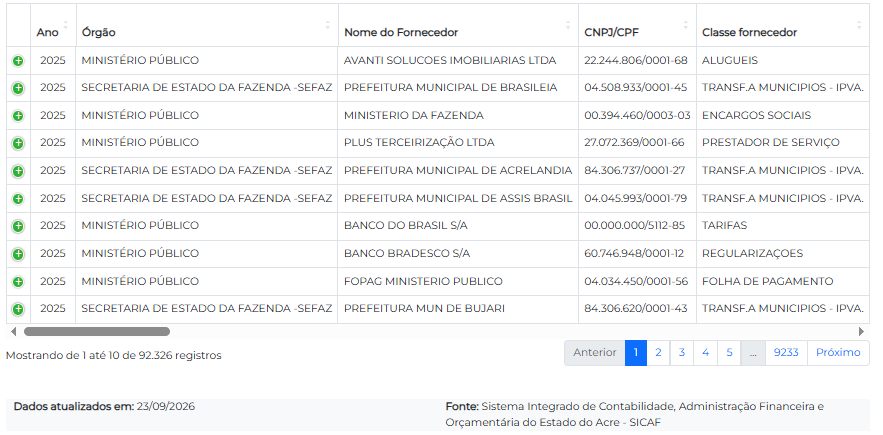
\includegraphics[width=0.95\textwidth]{PTGV.png}
    }{%
        \fbox{\parbox[c][3cm][c]{0.8\textwidth}{\centering \textbf{Imagem PTGV.png}\newline\small{arquivo ainda não adicionado em figures/}}}
    }
    \caption{Interface do Portal da Transparência evidenciando a disponibilização de microdados brutos de despesas governamentais.}
    \label{fig:portal_transparencia_excesso}
    \fonte{Governo do Estado do Acre (2026). Acesso em: 1 out. 2026 \cite{portal_despesas_acre2026}.}
\end{figure}

Como observado na Figura \ref{fig:portal_transparencia_excesso}, a consulta disponibiliza linhas com códigos orçamentários, favorecidos e históricos contábeis em texto livre. Examinar manualmente mais de 429 mil registros para localizar padrões que mereçam análise contextual — como pagamentos recorrentes, valores atípicos ou concentração de fornecedores — é operacionalmente inviável.

Nesse contexto, justifica-se a aplicação da \textbf{Ciência de Dados Forense} e do aprendizado de máquina não supervisionado. Em vez de exigir que o usuário navegue manualmente por tabelas extensas, a construção de um pipeline computacional automatizado atua como uma camada de inteligência analítica, capaz de triar a base populacional integral, reduzir o universo amostral de risco e apresentar sinalizadores preditivos (\textit{red flags}) para priorizar a investigação humana.

Diante dessa problemática, formula-se a seguinte \textbf{Pergunta de Pesquisa} que orienta este trabalho:\begin{quote}
\textit{Em que medida a aplicação de um pipeline de Ciência de Dados baseado em Aprendizado Não Supervisionado (\textit{Isolation Forest}, \textit{Local Outlier Factor} e \textit{DBSCAN}), testes de aderência à Lei de Benford e análise por $Z$-Score, combinados ao Processamento de Linguagem Natural, permite sinalizar e caracterizar padrões atípicos nos arquivos de despesas do Portal da Transparência do Estado do Acre (2020--2025), sem dados previamente rotulados?}
\end{quote}

\chapter{OBJETIVOS DA PESQUISA}\label{sec:objetivos}
Com o intuito de responder à pergunta de pesquisa formulada e viabilizar a análise computacional dos microdados abertos do setor público, este capítulo delimita o objetivo geral e os objetivos específicos que norteiam o desenvolvimento deste trabalho.

\section{Objetivo Geral}\label{sec:objetivo_geral}
Desenvolver e avaliar uma metodologia baseada em técnicas de Ciência de Dados e Aprendizado de Máquina para detectar padrões anômalos nas despesas públicas registradas no Portal da Transparência e relacionadas ao Estado do Acre, identificando transações ou grupos de transações que apresentem comportamento atípico em relação aos padrões históricos de execução da despesa.

\section{Objetivos Específicos}\label{sec:objetivos_especificos}
Para o alcance do objetivo geral, estabelecem-se os seguintes objetivos específicos:
\begin{enumerate}
    \item Coletar, integrar e organizar os dados de despesas públicas do Portal da Transparência do Acre, construindo o subconjunto de dados do estudo;
    \item Caracterizar estatisticamente o comportamento das despesas, avaliando sua distribuição, concentração, variabilidade e evolução temporal segundo órgão, favorecido e classificação da despesa;
    \item Mapear indicadores e atributos que expressem padrões potencialmente anômalos nas despesas, considerando valor, frequência, recorrência, concentração por favorecido e variação temporal;
    \item Aplicar métodos de análise não supervisionada para identificar observações ou padrões anômalos nas despesas analisadas;
    \item Comparar a concordância e a sensibilidade dos resultados a diferentes configurações dos procedimentos de detecção, identificando registros sinalizados por uma ou mais abordagens;
    \item Investigar a distribuição das anomalias identificadas segundo órgãos, favorecidos, categorias de despesa e períodos de execução, buscando reconhecer padrões socioadministrativos recorrentes;
    \item Desenvolver um escore ou classificação de prioridade das observações detectadas, de forma a auxiliar na seleção das despesas que mereçam atenção analítica;
    \item Avaliar a aplicabilidade da metodologia proposta como instrumento complementar de transparência e controle dos gastos públicos.
\end{enumerate}

\chapter{JUSTIFICATIVA DA PESQUISA}\label{sec:justificativa}

A relevância deste Trabalho de Conclusão de Curso fundamenta-se na interseção entre a Ciência de Dados, a Ciência da Informação e a Gestão Pública, desdobrando-se nas dimensões social, científica, técnica e prática.

\section{Relevância Social e Prática}\label{sec:relevancia_social}

A consolidação do princípio constitucional da publicidade e os avanços promovidos pela Lei de Acesso à Informação (Lei nº 12.527/2011) garantiram o direito fundamental de acesso aos dados orçamentários do setor público brasileiro. Contudo, a simples publicação de relatórios contábeis extensos e dados brutos nos portais de transparência não assegura, por si só, a efetividade da transparência pública. Na prática, a sociedade civil, jornalistas de dados e a comunidade acadêmica enfrentam o fenômeno da "opacidade por excesso" (\textit{information overload}), no qual o volume massivo e desestruturado de informações impede a compreensão direta sobre como os recursos públicos estão sendo alocados \cite{cavalcanti2014, pereira2025}.

Nesse contexto, a aplicação de técnicas de Ciência de Dados atua como um instrumento de democratização da informação e fortalecimento do controle social. Ao transformar microdados financeiros brutos em representações analíticas compreensíveis e padrões interpretáveis, a pesquisa contribui para reduzir a assimetria de informação entre a administração governamental e o cidadão. Além disso, no âmbito prático da gestão pública, o desenvolvimento de mecanismos abertos de triagem automatizada permite identificar gargalos normativos e padrões atípicos de execução orçamentária, fornecendo subsídios para o aprimoramento da eficiência administrativa e do planejamento de políticas públicas no Estado do Acre.

\section{Relevância Científica e Acadêmica}\label{sec:relevancia_cientifica}

Apesar da expansão de pesquisas dedicadas ao uso de técnicas computacionais e estatísticas na fiscalização de gastos públicos no Brasil, observa-se que a literatura científica nacional concentra suas aplicações predominantemente em dados federais — como o Cartão de Pagamento do Governo Federal (CPGF) e o SICONFI — ou em grandes metrópoles das regiões Sul e Sudeste \cite{cavalcanti2014, nunes2021}. Em contrapartida, o ecossistema de dados abertos dos entes subnacionais da Região Norte, em especial do Estado do Acre, permanece subexplorado pela pesquisa em Ciência de Dados e Sistemas de Informação.

O ineditismo regional desta pesquisa reside justamente na aplicação e validação de um pipeline computacional não supervisionado sobre a base populacional de despesas do Poder Executivo do Estado do Acre. Do ponto de vista científico, o estudo preenche uma lacuna relevante na literatura ao investigar como modelos de detecção de anomalias e testes estatísticos de distribuição comportam-se diante das especificidades orçamentárias, normativas e fornecedoras de uma unidade federativa da Amazônia Sul-Ocidental. Assim, o trabalho amplia a validade externa das metodologias de Ciência de Dados aplicadas à transparência pública, fornecendo um arcabouço metodológico reprodutível e replicável para outros estados com dinâmicas administrativas semelhantes \cite{pereira2025}.

\section{Relevância Técnica e Tecnológica}\label{sec:relevancia_tecnica}

Do ponto de vista tecnológico e computacional, a justificativa deste trabalho assenta-se na aplicação dos procedimentos analíticos a todas as linhas dos arquivos obtidos para o recorte temporal. Essa cobertura evita a seleção de uma amostra dentro dos arquivos reunidos, mas não garante que os arquivos representem todos os registros publicados pelo órgão nem que os métodos detectem todos os padrões atípicos. A completude será delimitada aos arquivos disponíveis e às regras de inclusão e exclusão descritas na metodologia.

Ademais, a arquitetura metodológica proposta responde a um desafio técnico central na mineração de dados abertos governamentais: a ausência de rótulos prévios (\textit{unlabelled data}). Ao integrar modelos de Aprendizado de Máquina Não Supervisionado (\textit{Isolation Forest}, \textit{Local Outlier Factor} e \textit{DBSCAN}) a testes estatísticos de distribuição (Lei de Benford e $Z$-Score) e técnicas de Processamento de Linguagem Natural (NLP), a pesquisa propõe um pipeline para sinalizar padrões atípicos e contextualizá-los à luz de regras normativas da administração pública \cite{cavalcanti2014, nunes2021, goldschmidt2005}. Trata-se de uma proposta metodológica orientada à triagem e à análise contextual dos dados.

\section{Viabilidade da Pesquisa}\label{sec:viabilidade}

A viabilidade técnica, operacional e temporal deste projeto de pesquisa é plenamente assegurada pela conjugação de três fatores fundamentais: a disponibilidade de dados públicos abertos, o uso de ecossistemas computacionais de código aberto (\textit{open-source}) e o avanço prévio do pipeline de dados.

Em primeiro lugar, o acesso aos arquivos públicos utilizados é compatível com a Lei de Acesso à Informação (Lei nº 12.527/2011) \cite{lai2011}. A transparência fiscal também é disciplinada pela Lei de Responsabilidade Fiscal (Lei Complementar nº 101/2000) \cite{lrf2000}. O estudo analisa os arquivos disponibilizados pelo Portal da Transparência do Estado do Acre, sem inferir que a publicidade dos dados dispense outras avaliações institucionais eventualmente aplicáveis.

Em segundo lugar, a exequibilidade computacional do trabalho apoia-se no uso da linguagem de programação Python e do seu ecossistema científico especializado (\textit{pandas}, \textit{numpy}, \textit{scikit-learn}, \textit{seaborn} e \textit{networkx}). A opção por bibliotecas abertas e consolidadas elimina a dependência de licenças de software proprietário de alto custo e assegura a transparência e a reprodutibilidade integral do pipeline analítico \cite{pereira2025}.

Por fim, a viabilidade cronológica é corroborada pela fase adiantada de preparação da base de dados. O processo de extração, limpeza e padronização do recorte populacional do Estado do Acre (2020--2025) — englobando mais de 429 mil registros financeiros — já se encontra concluído e validado em ambiente computacional. Esse amadurecimento técnico prévio mitiga riscos operacionais e assegura o cumprimento rigoroso do cronograma acadêmico estipulado para a execução do TCC.

\chapter{FUNDAMENTAÇÃO TEÓRICA}\label{sec:fundamentacao}

Neste capítulo, apresentam-se os conceitos teóricos, modelos estatísticos, algoritmos computacionais e estudos correlatos que sustentam o desenvolvimento desta pesquisa.

\section{Transparência Pública, Dados Abertos e Controle Social}\label{sec:transparencia_dados_abertos}

A consolidação da transparência na administração pública brasileira é resultado de um processo histórico de aperfeiçoamento institucional e normativo, impulsionado pela promulgação da Lei de Responsabilidade Fiscal (Lei Complementar nº 101/2000) e pela Lei de Acesso à Informação (Lei nº 12.527/2011 -- LAI). Esses marcos legalmente formalizaram a transição do modelo tradicional de sigilo administrativo para o paradigma da transparência ativa, no qual a publicidade passa a ser a regra geral e o sigilo, a exceção. Como decorrência, os entes federativos passaram a ser obrigados a disponibilizar, em portais de acesso público na internet, dados em tempo real sobre a execução orçamentária, financeira e operacional do setor público \cite{cavalcanti2014, pereira2025}.

Entretanto, a disponibilização bruta de dados nos portais de transparência governamentais expõe uma limitação crítica da transparência passiva e ativa não mediadas por ferramentas analíticas. Na literatura de Ciência da Informação e Gestão Pública, esse fenômeno é denominado "opacidade por excesso" (\textit{information overload}). A publicação de tabelas com centenas de milhares de linhas, caracterizadas por descrições contábeis genéricas, ausência de metadados consolidados e falta de filtros inteligentes, cria uma barreira cognitiva para o cidadão comum, para jornalistas de dados e para a comunidade acadêmica \cite{cavalcanti2014, nunes2021}. Embora o dado esteja formalmente acessível do ponto de vista jurídico, ele permanece ininteligível do ponto de vista prático e social.

A superação desse obstáculo é condição fundamental para o pleno exercício do controle social — mecanismo pelo qual a sociedade civil organizada participa da fiscalização e do acompanhamento da aplicação dos recursos públicos. Conforme destacado por Nunes \textit{et al.} (2021), a efetividade da transparência governamental não reside na mera exibição técnica de dados de despesas, mas na transformação desses microdados em conhecimento estruturado, capaz de apontar autonomamente comportamentos atípicos e sinalizar padrões de alocação de recursos que exijam análise aprofundada \cite{nunes2021}.

Assim, o uso da Ciência de Dados e de sistemas computacionais abertos posiciona-se como uma ponte entre a disponibilidade legal do dado público e o seu aproveitamento prático pelo controle social, viabilizando a automação do processo de triagem sobre bases populacionais volumosas sem depender exclusivamente de auditorias analógicas ou de conhecimento especializado contábil \cite{nunes2021, pereira2025}.

\section{O Processo KDD (\textit{Knowledge Discovery in Databases}) e a Análise Populacional}\label{sec:kdd_analise_populacional}

A extração de conhecimento a partir de grandes volumes de dados brutos exige a aplicação de metodologias estruturadas que orientem o tratamento da informação desde a sua coleta até a interpretação dos resultados. Na Ciência de Dados e na Mineração de Dados (\textit{Data Mining}), o modelo conceitual amplamente aceito para essa finalidade é o processo de Descoberta de Conhecimento em Bases de Dados (\textit{Knowledge Discovery in Databases} -- KDD) \cite{goldschmidt2005, pereira2025}.

O ciclo KDD caracteriza-se por ser uma abordagem iterativa e sequencial, composta por cinco etapas fundamentais \cite{goldschmidt2005}:
\begin{enumerate}
    \item \textbf{Seleção:} Identificação e extração do conjunto de dados relevante (\textit{dataset}) a partir das fontes operacionais brutas;
    \item \textbf{Pré-processamento e Limpeza:} Higienização da base mediante o tratamento de valores ausentes, remoção de inconsistências, eliminação de duplicatas e correção de ruídos de formatação;
    \item \textbf{Transformação:} Padronização dos tipos de dados, engenharia de atributos (\textit{feature engineering}) e adequação das variáveis para os formatos exigidos pelos algoritmos analíticos;
    \item \textbf{Mineração de Dados (\textit{Data Mining}):} Aplicação de modelos estatísticos e algoritmos computacionais para o mapeamento e extração de padrões, agrupamentos e anomalias;
    \item \textbf{Pós-processamento e Interpretação:} Validação, visualização e consolidação dos padrões descobertos em conhecimento útil e compreensível para o domínio de aplicação.
\end{enumerate}

No contexto desta pesquisa, o arcabouço KDD será aplicado a todas as linhas dos arquivos reunidos para o recorte definido. Essa análise cobre integralmente os arquivos utilizados, mas não permite afirmar que eles contenham todos os registros publicados pelo órgão. O processamento de todas as linhas evita a seleção de uma amostra dentro do conjunto coletado, sem eliminar limitações de cobertura, qualidade dos dados ou capacidade de detecção dos métodos \cite{pereira2025}.

O processamento uniforme das linhas dos arquivos coletados reduz a dependência de uma seleção amostral definida pelo pesquisador. O pipeline será usado como etapa de triagem para organizar registros com sinalizações de atipicidade e apoiar sua análise contextual; não assegura a identificação de todas as ocorrências relevantes nem substitui procedimentos de auditoria \cite{pereira2025}.

\section{Filtros Estatísticos de Distribuição: Lei de Benford e $Z$-Score}\label{sec:benford_zscore}

A análise da distribuição de frequências dos dígitos numéricos em bases de dados financeiras constitui uma técnica clássica da contabilidade forense e da Ciência de Dados para a identificação primária de anomalias estatísticas. O pilar fundamental dessa abordagem é a Lei de Newcomb-Benford (também conhecida como a Lei do Primeiro Dígito Significativo), descrita originalmente pelo astrônomo Simon Newcomb em 1881 e redescoberta pelo físico Frank Benford em 1938 \cite{nigrini2012, pereira2025}.

Diferentemente da intuição comum, que pressupõe uma distribuição uniforme na qual cada dígito de 1 a 9 teria 11,1\% de probabilidade de ocupar a primeira posição em um número, a Lei de Benford demonstra que dados numéricos decorrentes de fenômenos naturais, sociais e econômicos não manipulados obedecem a uma distribuição logarítmica. Matematicamente, a probabilidade $P(d)$ de um número iniciar com o dígito $d \in \{1, 2, \dots, 9\}$ é dada pela Equação \ref{eq:benford}:

\begin{equation}\label{eq:benford}
P(d) = \log_{10}\left(1 + \frac{1}{d}\right)
\end{equation}

Conforme essa distribuição, o dígito 1 possui a maior probabilidade teórica de ocorrência (aproximadamente $30,1\%$), enquanto o dígito 9 apresenta a menor probabilidade (aproximadamente $4,6\%$). Quando dados financeiros sofrem manipulação humana deliberada ou ajustes artificiais — como o fracionamento de compras para burlar limites de licitação (\textit{smurfing}) —, a distribuição natural dos dígitos tende a ser distorcida, gerando um desvio detectável frente à curva teórica \cite{nigrini2012, cavalcanti2014}.

Para avaliar a conformidade de uma base de dados pública frente à Lei de Benford, a literatura estabelece dois testes estatísticos complementares \cite{nigrini2012, pereira2025}:
\begin{enumerate}
    \item \textbf{Teste Qui-Quadrado ($\chi^2$):} Utilizado para testar a hipótese nula ($H_0$) de aderência global da base de dados, determinando se a distribuição observada dos dígitos desvia significativamente da distribuição teórica esperada em nível macro;
    \item \textbf{Teste $Z$-Score:} Empregado para avaliar o desvio atômico e localizado de cada dígito individualmente, medindo quantos desvios-padrão a frequência observada dista da frequência teórica de Benford.
\end{enumerate}

No entanto, a aplicação da Lei de Benford sobre microdados abertos da administração pública exige cautela analítica. Como ressalta Cavalcanti (2014), picos de frequência observados em dígitos específicos (medidos por $Z$-Scores elevados) não são suficientes, por si sós, para classificar transações como anômalas. No setor público, desvios estatísticos podem decorrer de regras de negócio e padronizações normativas — tais como concessões de diárias com valores fixados por decreto, reembolsos padronizados e tabelamento de auxílios. Portanto, Benford deve ser tratado como uma sinalização descritiva aplicada a um conjunto de valores, a ser interpretada em conjunto com o contexto administrativo; não identifica individualmente uma transação anômala \cite{cavalcanti2014, nunes2021}.

\section{Aprendizado de Máquina Não Supervisionado na Detecção de Anomalias}\label{sec:aprendizado_nao_supervisionado}

O Aprendizado de Máquina (\textit{Machine Learning}) é a subárea da Inteligência Artificial dedicada ao desenvolvimento de algoritmos capazes de extrair conhecimento, identificar padrões e tomar decisões de forma automatizada a partir de dados históricos \cite{goldschmidt2005}. No domínio da detecção de anomalias, as técnicas de aprendizado dividem-se fundamentalmente em duas abordagens: \textbf{supervisionadas} e \textbf{não supervisionadas} \cite{nunes2021}.

Nas abordagens supervisionadas (como \textit{Support Vector Machines} -- SVM, Árvores de Decisão e Regressão Logística), o modelo exige um conjunto de dados previamente rotulado (\textit{labelled dataset}), no qual cada registro é formalmente classificado entre "regular" ou "anômalo" (\textit{ground truth}). Contudo, como ressaltado por Nunes \textit{et al.} (2021), a aplicação de modelos supervisionados sobre dados de finanças públicas é inviável na prática, uma vez que os microdados abertos dos portais de transparência não possuem rotulagem prévia de auditoria \cite{nunes2021}.

Diante da ausência de rótulos, a extração de atipicidades fundamenta-se no \textbf{Aprendizado de Máquina Não Supervisionado} (\textit{Unsupervised Learning}). Essa abordagem assume que a imensa maioria dos registros da base representa transações normais e legítimas, enquanto as anomalias correspondem a observações raras que se distanciam estruturalmente do comportamento padrão \cite{goldschmidt2005, nunes2021}. Para a execução deste projeto, destacam-se dois algoritmos não supervisionados consolidados na literatura:

\subsection{\textit{Isolation Forest} (ISO)}

Proposto originalmente por Liu, Ting e Zhou (2008), o \textit{Isolation Forest} (ISO) adota uma abordagem distinta dos algoritmos tradicionais baseados em distância ou densidade. Em vez de construir perfis de dados normais para posterior identificação de desvios, o ISO foca no \textbf{isolamento explícito das anomalias} \cite{liu2008isolation}.

O algoritmo opera mediante a construção de um conjunto de árvores de decisão aleatórias (\textit{iTrees}). Em cada nó da árvore, uma variável é selecionada aleatoriamente, seguida pela escolha de um ponto de corte arbitrário entre os valores mínimo e máximo dessa variável. Como as anomalias possuem atributos quantitativos atípicos ou frequências reduzidas, elas exigem poucas partições para serem completamente isoladas nas folhas mais rasas da árvore \cite{liu2008isolation}.

Matematicamente, a pontuação de anomalia $s(x, n)$ de uma observação $x$ em uma base de tamanho $n$ é definida pela Equação \ref{eq:iso_score}:

\begin{equation}\label{eq:iso_score}
s(x, n) = 2^{-\frac{E(h(x))}{c(n)}}
\end{equation}

Em que $E(h(x))$ representa a média do comprimento do caminho de busca de $x$ ao longo da floresta de árvores, e $c(n)$ é a extensão média de busca sem sucesso em uma árvore binária de busca construída com $n$ nós. Quanto mais próximo de $1$ for o escore $s$, maior é a probabilidade de a observação constituir uma anomalia isolada \cite{liu2008isolation}. A grande vantagem do \textit{Isolation Forest} em relação a outros algoritmos não supervisionados reside na sua baixa complexidade computacional e linearidade ($O(n \log n)$), tornando-o altamente eficiente para o processamento de bases populacionais volumosas como a do Portal da Transparência do Acre \cite{liu2008isolation, pereira2025}.

\subsection{\textit{Local Outlier Factor} (LOF)}

Desenvolvido por Breunig \textit{et al.} (2000), o \textit{Local Outlier Factor} (LOF) é um algoritmo de detecção de anomalias baseado em densidade local que emprega a técnica dos $k$-vizinhos mais próximos ($k$-NN) \cite{breunig2000lof}. O pilar conceitual do LOF fundamenta-se na premissa de que a anomalia não deve ser definida apenas pela sua distância global ao centro da base, mas sim pelo seu grau de isolamento relativo em relação à densidade da sua vizinhança local \cite{breunig2000lof, vieira2019}.

Para cada ponto $p$ da base, o algoritmo calcula a sua densidade de acessibilidade local (\textit{local reachability density} -- $lrd_k(p)$), comparando-a subsequentemente com a densidade de acessibilidade média dos seus $k$-vizinhos mais próximos. A razão entre essas densidades determina o fator de \textit{outlier} local ($LOF_k(p)$), expresso pela Equação \ref{eq:lof_score}:

\begin{equation}\label{eq:lof_score}
LOF_k(p) = \frac{\sum_{o \in N_k(p)} \frac{lrd_k(o)}{lrd_k(p)}}{|N_k(p)|}
\end{equation}

Em que $N_k(p)$ representa o conjunto dos $k$-vizinhos mais próximos do ponto $p$. A interpretação do indicador LOF ocorre da seguinte forma \cite{breunig2000lof}:
\begin{itemize}
    \item $LOF \approx 1$: Indica que o ponto possui densidade similar à de seus vizinhos, pertencendo a um agrupamento denso e homogêneo (padrão normal);
    \item $LOF < 1$: Representa observações localizadas no interior de agrupamentos muito densos;
    \item $LOF \gg 1$: Sinaliza que a densidade do ponto é significativamente menor do que a de seus vizinhos, caracterizando-o como um \textit{outlier} local atípico.
\end{itemize}

A aplicação do LOF em dados da administração pública demonstra grande utilidade para identificar municípios ou órgãos cujos padrões de despesa destoam substancialmente de seus pares comparáveis (como demonstrado por Vieira, 2019 ao analisar repasses do SICONFI) \cite{vieira2019}. A integração combinada do \textit{Isolation Forest} e do \textit{Local Outlier Factor} permite capturar tanto anomalias globais quanto desvios locais de densidade na base orçamentária do Estado do Acre \cite{breunig2000lof, liu2008isolation}.

\section{Mineração de Texto em Históricos Contábeis (NLP e DBSCAN)}\label{sec:nlp_dbscan}

Enquanto os campos numéricos e cadastrais das despesas públicas possibilitam análises quantitativas diretas, a real intenção e o detalhamento das contratações governamentais residem no campo descritivo de texto livre, denominado \textbf{histórico do empenho/pagamento}. O tratamento analítico dessa variável impõe desafios adicionais à Ciência de Dados devido à ausência de padronização, presença de abreviações informais, ruídos de digitação e variações sintáticas \cite{goldschmidt2005, pereira2025}.

Para converter esse conteúdo textual não estruturado em representações numéricas computáveis, utiliza-se a técnica de vetorização por Frequência do Termo--Inverso da Frequência nos Documentos (\textit{Term Frequency--Inverse Document Frequency} -- TF-IDF). A métrica TF-IDF pondera a relevância de uma palavra $t$ em um histórico $d$ pertencente a um conjunto de documentos $D$, penalizando termos excessivamente genéricos (como "referente", "pago", "aquisição") e valorizando termos discriminativos (como nomes de insumos, medicamentos ou serviços específicos) \cite{goldschmidt2005}. Matematicamente, a ponderação é calculada pela Equação \ref{eq:tfidf}:

\begin{equation}\label{eq:tfidf}
\text{TF-IDF}(t, d, D) = \text{TF}(t, d) \times \log\left(\frac{|D|}{|\{d \in D : t \in d\}|}\right)
\end{equation}

Uma vez obtida a matriz esparsa de vetores TF-IDF, emprega-se o algoritmo de agrupamento baseado em densidade \textbf{DBSCAN} (\textit{Density-Based Spatial Clustering of Applications with Noise}), proposto por Ester \textit{et al.} (1996) \cite{ester1996dbscan}. Ao contrário de algoritmos de particionamento como o K-Means, o DBSCAN oferece três vantagens cruciais para a análise de despesas públicas \cite{ester1996dbscan, vieira2019}:
\begin{enumerate}
    \item Não exige a definição prévia do número de agrupamentos ($k$);
    \item Identifica agrupamentos de formatos geométricos arbitrários no espaço vetorial;
    \item Isola autonomamente pontos de ruído (\textit{noise}), isto é, históricos atípicos que não possuem densidade similar a nenhum grupo.
\end{enumerate}

O DBSCAN é parametrizado pelo raio de vizinhança ($\varepsilon$) e pelo número mínimo de pontos ($MinPts$). Neste estudo, a integração de TF-IDF com DBSCAN será usada para agrupar históricos com vocabulário semelhante e sinalizar descrições pouco próximas dos grupos encontrados. Como os arquivos não incluem quantidade contratada nem preço unitário, essa etapa não permitirá calcular variações de preço unitário ou concluir a ocorrência de fracionamento de licitação; poderá apenas orientar investigação contextual de recorrências e descrições relacionadas \cite{nunes2021}.

\section{Trabalhos Relacionados}\label{sec:trabalhos_relacionados}

A consolidação da Ciência de Dados Forense aplicada ao setor público é evidenciada por um conjunto crescente de estudos que investigam a detecção de anomalias em bases orçamentárias brasileiras. O Quadro \ref{qua:trabalhos_relacionados} sintetiza os principais trabalhos correlatos da literatura, destacando seus objetivos, métodos e a lacuna preenchida pelo presente TCC.

\begin{quadro}[htbp]
\centering
\small
\caption{Trabalhos relacionados na literatura nacional.}
\label{qua:trabalhos_relacionados}
\resizebox{\textwidth}{!}{%
\begin{tabular}{|p{3.2cm}|p{3.5cm}|p{4.2cm}|p{4.5cm}|}
\hline
\textbf{Autor / Documento} & \textbf{Domínio / Escopo} & \textbf{Metodologia Computacional} & \textbf{Diferencial / Foco Principal} \\ \hline
Cavalcanti (2014) \cite{cavalcanti2014} & Cartão Corporativo (CPGF) -- Governo Federal (2013) & Lei de Benford, Teste $Z$-Score, Qui-Quadrado e DAM & Validação jurídica e discricionariedade do uso de filtros estatísticos em auditorias do CPGF. \\ \hline
Cella (2018) \cite{cella2018} & Despesas Públicas Municipais -- Estado de Goiás & Lei de Newcomb-Benford e Testes de Aderência Estatística & Avaliação de conformidade em contas municipais e identificação de distorções em dígitos iniciais. \\ \hline
Vieira (2019) \cite{vieira2019} & Gastos Municipais -- SICONFI / DATASUS / FIRJAN & Algoritmo LOF (\textit{Local Outlier Factor}) e Framework KDD & Unificação de bases fiscais e indicadores sociais para redução de falsos positivos em prefeituras. \\ \hline
Asensi (2020) \cite{asensi2020} & Despesas Públicas Municipais & Mineração de Dados e Parametrização de Gastos & Parametrização de custos públicos e mapeamento de padrões atípicos de execução orçamentária. \\ \hline
Nunes \textit{et al.} (2021) \cite{nunes2021} & Cartão Corporativo (CPGF) -- Exercícios 2018--2019 & K-Means, Agrupamento Hierárquico e Redes Complexas & Detecção de anomalias sem rotulagem prévia em gastos federais via topologia de redes. \\ \hline
Pereira (2025) \cite{pereira2025} & Desembolsos Extraorçamentários -- Estado de Goiás (2024) & Pipeline KDD, Lei de Benford, $Z$-Score e Qui-Quadrado em Python & Validação populacional (100\% da base) do desvio no Dígito 1 como filtro inicial de triagem. \\ \hline
\citeonline{cordova2025} & Ciência de Dados e controle interno nos estados brasileiros & Aplicações de Ciência de Dados e trilhas de auditoria & Desafios de implementação nos estados brasileiros. \\ \hline
\citeonline{schiavon2019} & Dados abertos governamentais & Estudo aplicado de Ciência de Dados & Aplicação de Ciência de Dados a dados abertos governamentais. \\ \hline
\citeonline{silva_souza2021} & Dados da administração pública sobre gastos & Análise de possíveis anomalias & Estudo de possíveis anomalias em dados administrativos de gastos públicos. \\ \hline
\end{tabular}%
}
\fonte{Elaborado pelo autor com base na literatura correlata (2026).}
\end{quadro}

A análise conjunta dos nove trabalhos relacionados sintetizados no Quadro \ref{qua:trabalhos_relacionados} evidencia uma evolução metodológica clara: enquanto os estudos seminais (como Cavalcanti, 2014 e Cella, 2018) analisaram a distribuição dos dígitos segundo a Lei de Benford e aplicaram testes de aderência, pesquisas subsequentes avançaram para a integração de algoritmos não supervisionados de densidade (Vieira, 2019) e topologia de redes (Nunes \textit{et al.}, 2021), culminando na adoção de pipelines populacionais integrais em ambiente Python (Pereira, 2025) e no diagnóstico da maturidade do controle interno estadual.

A despeito desse panorama consolidado, constata-se uma lacuna no que tange à integração conjunta dessas técnicas (Benford, ISO, LOF e NLP) aplicada a bases populacionais subnacionais da Amazônia Sul-Ocidental, cenário que fundamenta a oportunidade e o ineditismo do presente estudo de caso no Estado do Acre.

\chapter{PROCEDIMENTOS METODOLÓGICOS}\label{sec:metodologia}

Neste capítulo, apresentam-se os procedimentos metodológicos, a caracterização da pesquisa, o ambiente computacional, as fontes de dados e o detalhamento do pipeline de Ciência de Dados desenvolvido para a execução do estudo de caso no Governo do Estado do Acre.

\section{Caracterização da Pesquisa}\label{sec:caracterizacao_pesquisa}

A condução deste trabalho fundamenta-se nas diretrizes da metodologia científica aplicada aos Sistemas de Informação e à Ciência de Dados, sendo classificada segundo quatro dimensões principais:

\begin{enumerate}
    \item \textbf{Quanto à Natureza:} Classifica-se como uma \textbf{pesquisa aplicada}, pois visa produzir conhecimento direcionado à solução de um problema prático e concreto da gestão pública: a automação da triagem de despesas atípicas e a mitigação da "opacidade por excesso" nos dados abertos governamentais \cite{cavalcanti2014, pereira2025};

    \item \textbf{Quanto à Abordagem do Problema:} Trata-se de uma \textbf{pesquisa quantitativa e computacional}. A análise apoia-se na extração de métricas numéricas, testes estatísticos de aderência (Lei de Benford, $Z$-Score e Qui-Quadrado) e algoritmos de Aprendizado de Máquina Não Supervisionado para o mapeamento de anomalias sobre bases de dados estruturadas \cite{goldschmidt2005, nunes2021};

    \item \textbf{Quanto aos Objetivos:} Caracteriza-se como uma \textbf{pesquisa exploratória e descritiva}. Exploratória ao investigar padrões não rotulados nos microdados orçamentários do Estado do Acre, e descritiva ao caracterizar detalhadamente a distribuição temporal, institucional e categórica das despesas e dos desvios identificados;

    \item \textbf{Quanto aos Procedimentos Analíticos:} Configura-se como um \textbf{estudo de caso computacional}, focado na infraestrutura de dados abertos e na execução orçamentária do Poder Executivo do Estado do Acre no período de 2020 a 2025.
\end{enumerate}

\section{Fonte de Dados, Recorte Populacional e Atributos}\label{sec:fonte_dados_atributos}

A execução do estudo de caso fundamenta-se na extração e estruturação dos microdados financeiros abertos disponibilizados pelo Poder Executivo do Estado do Acre, por meio do seu Portal da Transparência.

\subsection{Origem e Acesso aos Dados}\label{subsec:origem_dados}

Os arquivos tabulares foram baixados manualmente da página de despesas do Portal da Transparência do Estado do Acre, disponível em \url{https://transparencia.ac.gov.br/despesas/?ano=2025}, em 1º de outubro de 2026. O conjunto utilizado reúne os arquivos referentes aos exercícios de 2020 a 2025, disponibilizados publicamente pelo Governo do Estado do Acre. A coleta consistiu no download dos arquivos, sem uso de \textit{web scraping}. Para permitir a conferência do recorte, serão mantidos os arquivos originais utilizados e descritas as etapas de integração, limpeza e exclusão de registros. A Lei de Acesso à Informação estabelece o acesso público a informações de interesse coletivo, observadas as hipóteses legais de restrição \cite{lai2011}; a Lei de Responsabilidade Fiscal também disciplina a transparência da gestão fiscal \cite{lrf2000}. Os identificadores de pessoas físicas, quando presentes, serão usados apenas para vincular registros e não serão divulgados integralmente nos resultados; tabelas e gráficos apresentarão dados agregados ou identificadores mascarados. O estudo utiliza arquivos disponibilizados publicamente e não substitui eventual avaliação institucional ou ética aplicável ao trabalho.

\subsection{Recorte Populacional e Temporal}\label{subsec:recorte_populacional}

Diferentemente de abordagens que selecionam uma amostra dos arquivos reunidos, este trabalho processa as linhas dos arquivos baixados para os exercícios de \textbf{2020 a 2025}, que totalizam \textbf{430.067 registros} na versão atualmente analisada. Os valores empenhados, liquidados e pagos aparecem em colunas distintas de cada registro, não como três registros separados. O total descreve os arquivos obtidos e não deve ser interpretado como prova de que representam todos os registros existentes no Portal. Essa delimitação permite observar a evolução temporal das despesas, incluindo o período da pandemia da COVID-19 e transições de gestão administrativa na esfera estadual.

\subsection{Dicionário de Atributos e Seleção de Variáveis}\label{subsec:dicionario_attributos}

Os arquivos CSV contêm os campos originais listados no Quadro \ref{qua:atributos_dados}. Atributos como primeiro dígito, frequência por credor e razão de concentração são calculados posteriormente pelo pipeline a partir desses campos.

\begin{quadro}[htbp]
\centering
\small
\caption{Dicionário de atributos selecionados da base de despesas públicas do Estado do Acre.}
\label{qua:atributos_dados}
\resizebox{\textwidth}{!}{%
\begin{tabular}{|p{3.5cm}|p{4.0cm}|p{3.2cm}|p{4.5cm}|}
\hline
\textbf{Categoria} & \textbf{Nome da Variável} & \textbf{Tipo de Dado} & \textbf{Descrição e Aplicação no Pipeline} \\ \hline
\textbf{Financeira} & \texttt{valor\_empenho}, \texttt{valor\_liquidado}, \texttt{valor\_pago} & Numérico (valores monetários) & Valores registrados nas etapas de empenho, liquidação e pagamento. O primeiro dígito e as medidas estatísticas são derivados do campo analisado. \\ \hline
\textbf{Temporal} & \texttt{ano}, \texttt{data\_empenho} & Inteiro e data & Exercício e data do empenho; permitem ordenar os registros e analisar sua evolução temporal. \\ \hline
\textbf{Institucional} & \texttt{orgao} & Categórico (texto) & Órgão associado ao registro; usado para agrupar despesas por órgão. O arquivo não apresenta campo separado de unidade gestora ou código do órgão. \\ \hline
\textbf{Credor} & \texttt{nome\_credor}, \texttt{cnpj\_cpf}, \texttt{classe\_credor} & Texto e identificador & Nome, documento e classe do credor; permitem agrupar registros por favorecido e analisar recorrência e concentração. \\ \hline
\textbf{Identificação} & \texttt{numero\_empenho} & Identificador (texto) & Número do empenho, utilizado para identificar ou rastrear o registro. \\ \hline
\textbf{Classificação orçamentária} & \texttt{elemento\_\allowbreak{}despesa}, \texttt{elemento\_\allowbreak{}despesa\_\allowbreak{}descricao}, \texttt{fonte}, \texttt{funcao}, \texttt{funcao\_\allowbreak{}descricao}, \texttt{subfuncao}, \texttt{subfuncao\_\allowbreak{}descricao} & Códigos e descrições & Classificações e descrições orçamentárias disponíveis nos arquivos; podem apoiar agrupamentos comparáveis de despesas. \\ \hline
\textbf{Textual} & \texttt{historico} & Texto livre & Histórico descritivo do empenho; pode ser processado por técnicas de NLP, como TF-IDF. \\ \hline
\end{tabular}%
}
\fonte{Elaborado pelo autor com base nos dados do Portal da Transparência do Estado do Acre (2026).}
\end{quadro}

\section{Estrutura do Pipeline Analítico}\label{sec:estrutura_pipeline}

Para a fase de execução e implementação da proposta, a metodologia do trabalho integrará os seguintes pilares analíticos:\begin{enumerate}
    \item \textbf{Filtro Estatístico Paramétrico (Lei de Benford e $Z$-Score):} Utilizado como linha de base estatística para analisar a distribuição natural dos dígitos financeiros e identificar padronizações normativas, tais como a concentração de valores tabelados em diárias operacionais e auxílios institucionais \cite{cavalcanti2014, nigrini2012};
    \item \textbf{Algoritmos Não Supervisionados de Detecção de Anomalias:} Aplicação planejada dos algoritmos \textit{Isolation Forest} (ISO) \cite{liu2008isolation} e \textit{Local Outlier Factor} (LOF) \cite{breunig2000lof} para o isolamento computacional de desvios e pontos discrepantes na distribuição dos gastos;
    \item \textbf{Mineração de Texto e Agrupamento (NLP e DBSCAN):} Emprego de técnicas de Processamento de Linguagem Natural combinadas com algoritmos de agrupamento baseados em densidade para analisar os históricos contábeis e identificar contratos continuados em serviços essenciais;
    \item \textbf{Representação Relacional Complementar:} Uso exploratório de redes para descrever relações observadas entre órgãos e credores; padrões de conexão serão tratados como hipóteses para análise contextual, não como evidência de coordenação entre fornecedores \cite{nunes2021}.
\end{enumerate}
Dessa forma, esta pesquisa contribui para a literatura de Ciência de Dados Aplicada ao demonstrar como técnicas computacionais não supervisionadas podem servir como instrumentos de inteligência institucional, revelando dinâmicas organizacionais, gargalos normativos e padrões de alocação de recursos no Estado do Acre.

Para superar os gargalos da fiscalização analógica e converter grandes massas de dados orçamentários em inteligência fiscal, este trabalho propõe um pipeline computacional estruturado nas etapas do processo de Descoberta de Conhecimento em Bases de Dados (\textit{Knowledge Discovery in Databases} -- KDD). A Figura \ref{fig:fluxograma_kdd} ilustra a arquitetura geral do fluxo de processamento analítico desenvolvido.

\begin{figure}[htbp]
    \centering
    \caption{Fluxograma geral da esteira de Ciência de Dados Forense baseada no ciclo KDD.}
    \label{fig:fluxograma_kdd}
    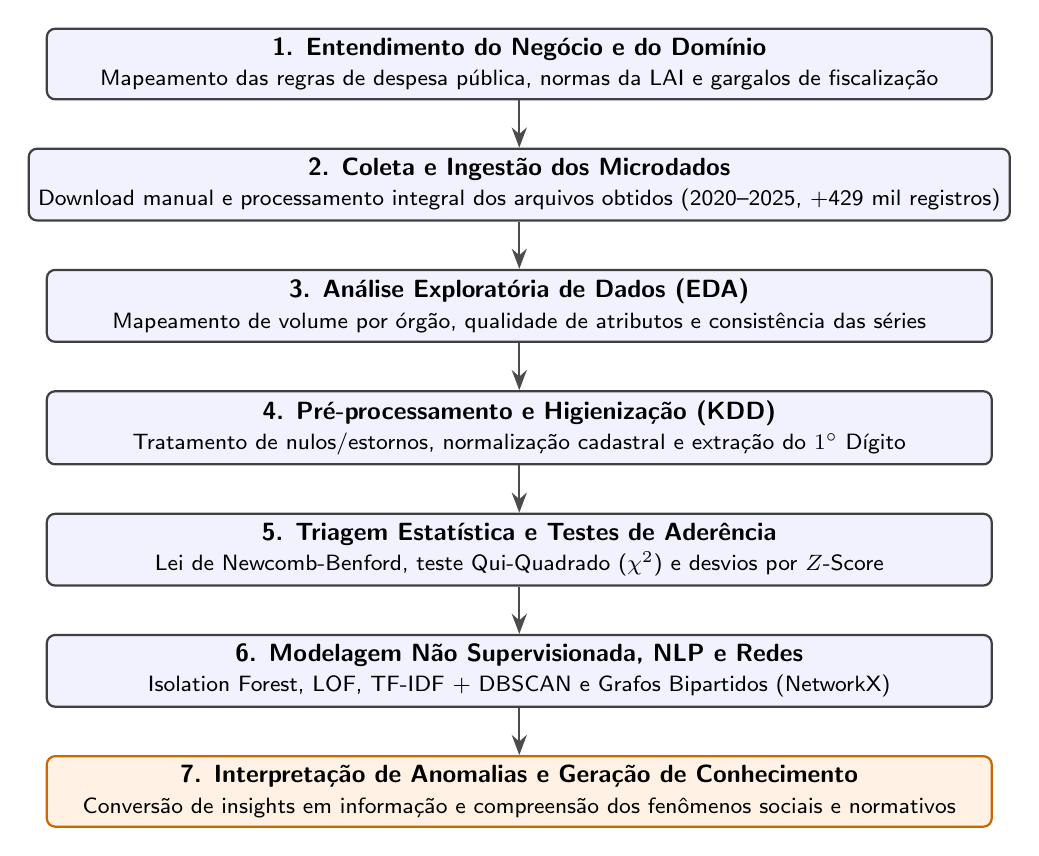
\begin{tikzpicture}[
        node distance=0.6cm and 1.0cm,
        box/.style={
            rectangle,
            draw=black!75,
            fill=blue!5,
            thick,
            rounded corners=3pt,
            align=center,
            font=\small\sffamily,
            minimum width=12cm,
            minimum height=0.8cm
        },
        boxfinal/.style={
            rectangle,
            draw=orange!80!black,
            fill=orange!10,
            thick,
            rounded corners=3pt,
            align=center,
            font=\small\sffamily,
            minimum width=12cm,
            minimum height=0.8cm
        },
        arrow/.style={
            -{Stealth[scale=1.1]},
            thick,
            draw=black!70
        }
    ]
        \node (fase1) [box] {\textbf{1. Entendimento do Negócio e do Domínio} \\ {\footnotesize Mapeamento das regras de despesa pública, normas da LAI e gargalos de fiscalização}};
        \node (fase2) [box, below=of fase1] {\textbf{2. Coleta e Ingestão dos Microdados} \\ {\footnotesize Download manual e processamento integral dos arquivos obtidos (2020--2025, +429 mil registros)}};
        \node (fase3) [box, below=of fase2] {\textbf{3. Análise Exploratória de Dados (EDA)} \\ {\footnotesize Mapeamento de volume por órgão, qualidade de atributos e consistência das séries}};
        \node (fase4) [box, below=of fase3] {\textbf{4. Pré-processamento e Higienização (KDD)} \\ {\footnotesize Tratamento de nulos/estornos, normalização cadastral e extração do $1^{\circ}$ Dígito}};
        \node (fase5) [box, below=of fase4] {\textbf{5. Triagem Estatística e Testes de Aderência} \\ {\footnotesize Lei de Newcomb-Benford, teste Qui-Quadrado ($\chi^2$) e desvios por $Z$-Score}};
        \node (fase6) [box, below=of fase5] {\textbf{6. Modelagem Não Supervisionada, NLP e Redes} \\ {\footnotesize Isolation Forest, LOF, TF-IDF + DBSCAN e Grafos Bipartidos (NetworkX)}};
        \node (fase7) [boxfinal, below=of fase6] {\textbf{7. Interpretação de Anomalias e Geração de Conhecimento} \\ {\footnotesize Conversão de insights em informação e compreensão dos fenômenos sociais e normativos}};

        \draw [arrow] (fase1) -- (fase2);
        \draw [arrow] (fase2) -- (fase3);
        \draw [arrow] (fase3) -- (fase4);
        \draw [arrow] (fase4) -- (fase5);
        \draw [arrow] (fase5) -- (fase6);
        \draw [arrow] (fase6) -- (fase7);
    \end{tikzpicture}
    \fonte{Elaborado pelo autor (2026).}
\end{figure}

A execução da esteira inicia-se pela compreensão das normas de execução orçamentária do setor público (Fase 1), seguida do download manual dos arquivos de despesas disponibilizados pelo Estado do Acre para 2020 a 2025 e do processamento integral das linhas contidas nesses arquivos (Fase 2). Essa etapa não pressupõe que os arquivos obtidos correspondam à totalidade dos registros publicados pelo Portal. Após a verificação exploratória de consistência (Fase 3) e o pré-processamento para limpeza de ruídos e extração de atributos numéricos (Fase 4), os dados passam pela análise da distribuição dos dígitos e por testes de aderência relacionados à Lei de Benford e ao $Z$-Score (Fase 5).

Na sequência, aplicam-se modelos não supervisionados de isolamento e densidade (\textit{Isolation Forest} e LOF), técnicas de mineração de texto (TF-IDF e DBSCAN) e modelagem de redes complexas para identificar atipicidades quantitativas, semânticas e relacionais (Fase 6). Por fim, a Fase 7 dedica-se à conversão dos outputs algorítmicos em conhecimento estruturado, promovendo a interpretação contextual dos resultados para compreender os fenômenos sociais, econômicos e normativos subjacentes às anomalias detectadas.

\section{A Esteira de Processamento de Dados (Pipeline KDD)}\label{sec:pipeline_kdd}

O processamento analítico dos microdados orçamentários do Estado do Acre segue rigorosamente as etapas do ciclo de Descoberta de Conhecimento em Bases de Dados (\textit{Knowledge Discovery in Databases} -- KDD) \cite{goldschmidt2005, pereira2025}. A esteira computacional foi estruturada modularmente em ambiente Python, articulando tratamentos estatísticos e modelos de algoritmos não supervisionados.

\subsection{Pré-processamento e Higienização de Dados (\textit{Data Cleaning})}\label{subsec:limpeza_dados}

A etapa inicial de pré-processamento foca na transformação dos arquivos brutos em uma estrutura tabular uniforme e livre de ruídos que possam comprometer a convergência dos algoritmos \cite{goldschmidt2005}. Executam-se as seguintes rotinas computacionais:

\begin{enumerate}
    \item \textbf{Tratamento de Valores Nulos e Inconsistentes:} Mapeamento e imputação/remoção de registros com variáveis essenciais ausentes (\texttt{NaN}), tais como valores zerados de empenho ou códigos de credor inconsistentes;
    \item \textbf{Normalização de Identificadores Cadastrais:} Limpeza de caracteres especiais (pontos, traços e barras) nos campos de CPF e CNPJ dos favorecidos, aplicando preenchimento com zeros à esquerda (\textit{zfill}) para garantir o padrão numérico de 11 e 14 dígitos;
    \item \textbf{Tratamento de Estornos e Operações Negativas:} Conversão dos valores contábeis de anulação e estorno para o seu módulo absoluto ($|x|$), rotulando a natureza da transação para evitar distorções nas métricas agregadas de despesa acumulada;
    \item \textbf{Padronização Temporal e Textual:} Conversão de datas para o formato padrão ISO 8601 (\texttt{YYYY-MM-DD}) e conversão de todo o texto dos históricos de empenho para caracteres minúsculos, removendo acentuação e pontuação desnecessária.
\end{enumerate}

\subsection{Engenharia de Atributos (\textit{Feature Engineering})}\label{subsec:feature_engineering}

Nesta fase, constroem-se novas variáveis sintéticas a partir dos atributos brutos, com o objetivo de capturar comportamentos atípicos e fornecer insumos específicos para os modelos quantitativos e qualitativos \cite{pereira2025}:

\begin{enumerate}
    \item \textbf{Extração do Primeiro Dígito Significativo (\texttt{primeiro\_digito}):} Isolamento do primeiro dígito diferente de zero de cada valor financeiro positivo selecionado, variável derivada para a análise de Benford;
    \item \textbf{Frequência Recorrente por Favorecido (\texttt{freq\_credor}):} Contagem automatizada do número de empenhos e liquidações emitidos para um mesmo CNPJ/CPF em janelas temporais de 30, 60 e 90 dias;
    \item \textbf{Razão de Concentração do Favorecido (\texttt{razao\_concentracao}):} Percentual do total registrado para um órgão direcionado a um único credor no exercício financeiro;
    \item \textbf{Variabilidade da Despesa (\texttt{desvio\_relativo}):} Razão entre o valor de uma transação específica e a média histórica de pagamentos do mesmo elemento de despesa no órgão.
\end{enumerate}

\subsection{Módulo Estatístico Paramétrico: Lei de Benford e $Z$-Score}\label{subsec:modulo_benford}

O primeiro filtro analítico atua sobre o primeiro dígito significativo dos valores positivos de cada campo financeiro, analisado separadamente. Valores nulos e negativos não têm primeiro dígito significativo e serão excluídos desse teste; a quantidade considerada e excluída será informada nos resultados. A aderência da distribuição observada é avaliada pelos testes a seguir \cite{nigrini2012, cavalcanti2014}:

\begin{enumerate}
    \item \textbf{Teste Qui-Quadrado ($\chi^2$):} Avalia a aderência global da distribuição observada à distribuição teórica de Benford. Para nove categorias de dígitos, o teste utiliza oito graus de liberdade e nível de significância $\alpha = 0,05$;
    \item \textbf{Teste $Z$-Score para Dígitos Individuais:} Avalia, para cada dígito de $1$ a $9$, o desvio entre a frequência observada e a esperada. O cálculo é regido pela Equação \ref{eq:z_score_formula}:
    \begin{equation}\label{eq:z_score_formula}
    Z_d = \frac{|p_o - p_e| - \frac{1}{2n}}{\sqrt{\frac{p_e (1 - p_e)}{n}}}
    \end{equation}
    Em que $p_o$ é a proporção observada do dígito $d$, $p_e$ é a proporção esperada por Benford e $n$ é o total de valores válidos. O termo $\frac{1}{2n}$ corresponde à correção de continuidade. Valores de $Z_d > 2,57$ serão tratados como sinalizações nominais de desvio em teste bilateral. Para as conclusões inferenciais sobre os nove dígitos, os valores-$p$ serão ajustados pelo procedimento de Holm--Bonferroni, com nível familiar de $1\%$ \cite{nigrini2012}.
\end{enumerate}

\subsection{Módulo de Aprendizado de Máquina Não Supervisionado: ISO e LOF}\label{subsec:modulo_ml}

Para superar a dependência de análises unidimensionais e identificar anomalias multivariadas complexas em dados não rotulados, o pipeline aplica concorrentemente dois algoritmos de Aprendizado Não Supervisionado \cite{nunes2021}:

\begin{enumerate}
    \item \textbf{\textit{Isolation Forest} (ISO):} Treinado sobre o vetor de atributos quantitativos (valor, frequência e razão de concentração), com \textit{contamination} igual a $0,01$ e \texttt{random\_state=42}. Uma observação recebe sinalização quando o modelo a classifica como outlier. O parâmetro \textit{contamination} define o limiar de decisão do modelo e não é uma probabilidade de que o registro seja anômalo \cite{liu2008isolation};
    \item \textbf{\textit{Local Outlier Factor} (LOF):} Executado separadamente por órgão, com hiperparâmetro de vizinhança $k = 20$ e variáveis numéricas padronizadas. Registros com escore $LOF > 1,5$ recebem sinalização de baixa densidade local \cite{breunig2000lof}.
\end{enumerate}

\subsection{Módulo de NLP e Agrupamento Semântico (TF-IDF + DBSCAN)}\label{subsec:modulo_nlp}

Como etapa de análise contextual, o campo original \texttt{historico} passa por um pipeline de Processamento de Linguagem Natural \cite{goldschmidt2005, ester1996dbscan}:

\begin{enumerate}
    \item \textbf{Vetorização TF-IDF:} Remoção de \textit{stopwords} em português e construção da matriz esparsa de relevância de termos, limitando-se às 1.000 palavras mais discriminativas;
    \item \textbf{Agrupamento com DBSCAN:} Aplicação do algoritmo DBSCAN sobre a matriz TF-IDF normalizada pela norma L2, utilizando distância do cosseno, raio $\varepsilon = 0,3$ e $MinPts = 5$. Observações rotuladas como ruído (\textit{label} $-1$) recebem uma sinalização de texto menos semelhante aos agrupamentos encontrados. Essa sinalização requer interpretação contextual e não caracteriza, por si só, uma anomalia administrativa \cite{ester1996dbscan, vieira2019}.
\end{enumerate}

\subsection{Análise de Sensibilidade dos Parâmetros}\label{subsec:analise_sensibilidade}


Como não há rótulos de auditoria para medir acurácia, a robustez da triagem será examinada variando um parâmetro por vez em torno da configuração de referência. Para o \textit{Isolation Forest}, serão comparados valores de \textit{contamination} de $0,005$, $0,01$ e $0,02$; para o LOF, limites de sinalização de $1,5$ e $2,0$, mantendo $k=20$; e, para o DBSCAN, $\varepsilon$ de $0,2$, $0,3$ e $0,4$, mantendo $MinPts=5$. Também serão comparadas regras de consenso de um, dois e três métodos sinalizadores. Para cada configuração, serão apresentados o número e a proporção de registros sinalizados, a interseção entre os conjuntos de candidatos e o índice de Jaccard em relação à configuração de referência ($0,01$, $LOF>1,5$, $\varepsilon=0,3$ e consenso de dois métodos). Essa análise avalia a estabilidade das sinalizações em relação aos parâmetros, não a acurácia em relação a uma verdade de referência.

Os parâmetros de referência são escolhas operacionais para a triagem, não limites universais nem estimativas da prevalência real de anomalias. O \textit{contamination} de $0,01$ fixa o limiar de decisão inicial do \textit{Isolation Forest}; no LOF, $1,5$ funciona como limiar heurístico para sinalizar densidade local suficientemente distinta da vizinhança; no DBSCAN, $\varepsilon=0,3$ define a distância máxima de cosseno entre observações vizinhas e $MinPts=5$ exige densidade mínima para formar um agrupamento. A regra de consenso de dois entre três métodos foi escolhida como critério intermediário: uma sinalização isolada é mais inclusiva, enquanto exigir unanimidade é mais restritivo.

\section{Análise de Redes Complexas e Topologia de Grafos}\label{sec:redes_complexas}

Para além das abordagens estatísticas e algoritmos atômicos de amostragem, a estrutura de contratação pública do Estado do Acre apresenta uma dimensão relacional intrínseca: a conexão entre entes governamentais (órgãos/secretarias) e fornecedores privados (empresas/favorecidos). Para mapear essa dinâmica, o pipeline incorpora a \textbf{Teoria dos Grafos e a Análise de Redes Complexas} \cite{nunes2021}.

\subsection{Modelagem de Rede Bipartida e Projeção}\label{subsec:rede_bipartida}

A relação entre órgãos e credores é representada por um grafo bipartido $G = (V_{org}, V_{cred}, E)$, em que $V_{org}$ representa os nós dos órgãos, $V_{cred}$ os nós dos credores/fornecedores e $E$ as relações observadas nos registros. As arestas poderão ser ponderadas pelo valor financeiro agregado ou pela quantidade de empenhos, conforme a unidade de análise definida na implementação:

\begin{enumerate}
    \item \textbf{Mapeamento Bipartido:} Construção da matriz de adjacência $A$, conectando cada secretaria aos seus respectivos fornecedores contratados;
    \item \textbf{Projeção Unimodal de Credores:} Projeção do grafo sobre o conjunto $V_{cred}$, conectando credores associados aos mesmos órgãos no período analisado. A coocorrência poderá orientar hipóteses sobre padrões de fornecimento e dependência administrativa, mas não evidencia, por si só, consórcios, coordenação entre empresas ou compartilhamento de contratos.
\end{enumerate}

\subsection{Métricas de Centralidade e Concentração de Fornecedores}\label{subsec:metricas_centralidade}

Para descrever a estrutura relacional dos fornecedores nos arquivos do estudo, serão calculadas duas métricas de rede via biblioteca \texttt{networkx} \cite{nunes2021}:

\begin{enumerate}
    \item \textbf{Centralidade de Grau (\textit{Degree Centrality}):} Mede o número de órgãos estaduais distintos atendidos por uma mesma empresa, identificando fornecedores hiperconectados na estrutura administrativa;
    \item \textbf{Centralidade de Intermediação (\textit{Betweenness Centrality}):} Quantifica a frequência com que um credor atua como ponte de conexão no fluxo de empenhos entre diferentes setores governamentais.
\end{enumerate}

Essa modelagem relacional permite descrever a concentração e a conectividade dos fornecedores, inclusive em situações de uso compartilhado de Atas de Registro de Preços ("caronas" interinstitucionais). Centralidade elevada é uma característica da rede e, isoladamente, não demonstra direcionamento ou captura de mercado.

\section{Ambiente Computacional e Ferramentas}\label{sec:ambiente_computacional}

A construção e execução do pipeline analítico utilizam linguagens e bibliotecas de código aberto (\textit{open-source}), reduzindo custos de licenciamento e favorecendo a inspeção e a reprodutibilidade do código. A Tabela \ref{tab:ambiente_ferramentas} detalha o ambiente computacional previsto:

\begin{table}[htbp]
\centering
\small
\caption{Ambiente computacional e bibliotecas especializadas utilizadas na pesquisa.}
\label{tab:ambiente_ferramentas}
\resizebox{\textwidth}{!}{%
\begin{tabular}{|p{3.5cm}|p{3.8cm}|p{8.0cm}|}
\hline
\textbf{Camada} & \textbf{Tecnologia / Biblioteca} & \textbf{Finalidade e Aplicação no Pipeline} \\ \hline
\textbf{Linguagem Base} & Python 3.10+ & Linguagem de programação científica para processamento e modelagem de dados. \\ \hline
\textbf{Manipulação de Dados} & \texttt{pandas} / \texttt{numpy} & Leitura de arquivos tabulares, limpeza, filtragem populacional e engenharia de atributos. \\ \hline
\textbf{Estatística Forense} & \texttt{scipy.stats} / \texttt{statsmodels} & Execução dos testes Qui-Quadrado ($\chi^2$), cálculo de $Z$-Score e distribuições de Benford. \\ \hline
\textbf{Machine Learning} & \texttt{scikit-learn} & Implementação dos algoritmos \textit{Isolation Forest}, \textit{Local Outlier Factor} (LOF), DBSCAN e TF-IDF. \\ \hline
\textbf{Análise de Redes} & \texttt{networkx} / \texttt{pyvis} & Modelagem topológica de grafos bipartidos e visualização interativa de redes de fornecedores. \\ \hline
\textbf{Visualização} & \texttt{matplotlib} / \texttt{seaborn} & Geração de gráficos de distribuição, histogramas de dígitos e curvas de aderência. \\ \hline
\textbf{Ambiente e Controle} & Google Colab / GitHub & Nuvem computacional de execução analítica e versionamento de código-fonte. \\ \hline
\end{tabular}%
}
\fonte{Elaborado pelo autor (2026).}
\end{table}

\section{Escore de Prioridade e Análise Contextual}\label{sec:escore_risco_validacao}

O escore tem a finalidade de ordenar registros para análise, não de estimar a probabilidade de uma anomalia. Ele combina apenas sinalizações produzidas por métodos aplicados a registros individuais. A Lei de Benford, por avaliar distribuições de conjuntos de valores, e as métricas de rede, por descreverem relações entre órgãos e credores, são analisadas separadamente como contexto.

\subsection{Composição do Escore Integrado}\label{subsec:composicao_escore}

Combinar detectores de outliers com princípios distintos é uma estratégia discutida na literatura de ensembles para reunir sinais potencialmente complementares; seu desempenho, porém, depende dos dados e dos métodos escolhidos \cite{aggarwal_sathe2017}. Neste estudo, adota-se uma votação simples, com peso igual para os três detectores, como regra operacional de priorização, não como reprodução de um escore definido por essa fonte.

Para cada registro $i$, cada um dos três métodos individuais produz uma sinalização binária: $S_{\text{ISO}}(i)=1$ quando o \textit{Isolation Forest} classifica o registro como outlier; $S_{\text{LOF}}(i)=1$ quando seu escore LOF é maior que $1,5$; e $S_{\text{DBSCAN}}(i)=1$ quando o histórico recebe o rótulo de ruído $-1$. Nos demais casos, o indicador vale zero. O escore é a proporção de métodos que sinalizaram o registro, convertida para a escala de 0 a 100:

\begin{equation}\label{eq:escore_risco}
R_i = \frac{100}{3}\left(S_{\text{ISO}}(i) + S_{\text{LOF}}(i) + S_{\text{DBSCAN}}(i)\right)
\end{equation}

Assim, $R_i$ pode assumir os valores $0$, $33,3$, $66,7$ ou $100$. Um registro é definido operacionalmente como \textbf{candidato a anomalia} quando pelo menos dois dos três métodos o sinalizam ($R_i \geq 66,7$). Registros com apenas uma sinalização permanecem como alertas individuais para análise exploratória. Esses limiares são regras de triagem do estudo, não comprovam a ocorrência de uma anomalia nem medem a acurácia dos métodos.

\subsection{Análise Contextual dos Candidatos}\label{subsec:validacao_falsos_positivos}

A etapa contextual examina os candidatos a anomalia à luz das informações disponíveis nos históricos, classificações orçamentárias e documentos normativos ou contratuais que puderem ser consultados. Cada caso será registrado como (a) explicado por regra ou contexto identificado, (b) atipicidade sem explicação encontrada nas fontes consultadas, ou (c) inconclusivo por falta de informação. Essa análise descreve os resultados da triagem; não confirma a ocorrência de conduta indevida nem substitui a apuração dos órgãos de controle \cite{cavalcanti2014, nunes2021}.

\chapter{CRONOGRAMA}\label{sec:cronograma}
O semestre letivo começa em 26 de outubro de 2026. Considerando o encerramento previsto, ainda não oficial, em 5 de maio de 2027, a defesa foi programada para 5 de abril de 2027, exatamente 30 dias antes. A Tabela \ref{tab:cronograma_atividades} apresenta as atividades em dias corridos; a Figura \ref{fig:gantt_cronograma} mostra sua distribuição no calendário, com o recesso acadêmico e a continuidade de atividades de pesquisa durante o período de férias acadêmicas. Se a data oficial de encerramento for diferente, a data da defesa deverá ser ajustada para manter esse intervalo.

\begin{table}[htbp]
\centering
\small
\caption{Cronograma de atividades do semestre letivo 2026.2, em dias corridos.}
\label{tab:cronograma_atividades}
\resizebox{\textwidth}{!}{%
\begin{tabular}{|p{2.5cm}|p{3.4cm}|c|p{8.0cm}|}
\hline
\textbf{Mês} & \textbf{Data} & \textbf{Dias} & \textbf{Atividade} \\ \hline
Outubro/\allowbreak Novembro & 26/10/2026--08/11/2026 & 14 & Ajustes do projeto e preparação do ambiente computacional. \\ \hline
Novembro & 09/11/2026--29/11/2026 & 21 & Expansão bibliográfica e desenvolvimento do Capítulo 2. \\ \hline
Novembro/\allowbreak Dezembro & 30/11/2026--22/12/2026 & 23 & Desenvolvimento do Capítulo 3 e organização da base de dados. \\ \hline
Dezembro/\allowbreak Janeiro & 23/12/2026--02/01/2027 & 11 & Recesso acadêmico. \\ \hline
Janeiro & 04/01/2027--17/01/2027 & 14 & Revisão bibliográfica complementar e aprofundamento do referencial teórico. \\ \hline
Janeiro & 18/01/2027--31/01/2027 & 14 & Documentação e validação da base, incluindo conferência de campos, nulos e duplicidades. \\ \hline
Fevereiro & 01/02/2027--15/02/2027 & 15 & Ajustes do pipeline e testes piloto para preparar os experimentos computacionais. \\ \hline
Fevereiro/\allowbreak Março & 16/02/2027--07/03/2027 & 20 & Execução dos experimentos computacionais. \\ \hline
Março & 08/03/2027--19/03/2027 & 12 & Tabulação dos resultados e produção das visualizações. \\ \hline
Março & 20/03/2027--29/03/2027 & 10 & Redação do Capítulo 4 e discussão dos resultados. \\ \hline
Março/\allowbreak Abril & 30/03/2027--04/04/2027 & 6 & Revisão da orientadora, ajustes e preparação da defesa. \\ \hline
Abril & 05/04/2027 & 1 & Defesa perante a banca. \\ \hline
Abril/\allowbreak Maio & 06/04/2027--05/05/2027 & 30 & Correções pós-banca e entrega da versão final. \\ \hline
\end{tabular}%
}
\fonte{Elaboração própria (2026).}
\end{table}

\begin{figure}[htbp]
    \centering
    \caption{Cronograma de execução da pesquisa, de 26 de outubro de 2026 a 5 de maio de 2027.}
    \label{fig:gantt_cronograma}

    \resizebox{\textwidth}{!}{%
    \begin{ganttchart}[
        time slot format=isodate,
        x unit=0.8mm,
        y unit title=0.6cm,
        y unit chart=0.55cm,
        vgrid,
        hgrid,
        title label font=\bfseries\scriptsize,
        bar label font=\scriptsize,
        bar/.style={fill=blue!20, draw=blue!70, line width=1pt, rounded corners=2pt},
        bar height=0.5,
        progress label text={},
        group right shift=0,
        group top shift=.6,
        group height=.3
    ]{2026-10-26}{2027-05-05}

    \gantttitlecalendar{year} \\
    \gantttitle{Out.}{6}\gantttitle{Novembro}{30}\gantttitle{Dezembro}{31}\gantttitle{Janeiro}{31}\gantttitle{Fevereiro}{28}\gantttitle{Março}{31}\gantttitle{Abril}{30}\gantttitle{Mai}{5} \\

    \ganttbar{Ajustes do projeto e ambiente (14 dias)}{2026-10-26}{2026-11-08} \\
    \ganttbar{Bibliografia e Capítulo 2 (21 dias)}{2026-11-09}{2026-11-29} \\
    \ganttbar{Capítulo 3 e base de dados (23 dias)}{2026-11-30}{2026-12-22} \\
    \ganttbar{Recesso acadêmico (11 dias)}{2026-12-23}{2027-01-02} \\
    \ganttbar{Revisão bibliográfica complementar (14 dias)}{2027-01-04}{2027-01-17} \\
    \ganttbar{Documentação e validação da base (14 dias)}{2027-01-18}{2027-01-31} \\
    \ganttbar{Ajustes do pipeline e testes piloto (15 dias)}{2027-02-01}{2027-02-15} \\
    \ganttbar{Experimentos computacionais (20 dias)}{2027-02-16}{2027-03-07} \\
    \ganttbar{Tabulação e visualizações (12 dias)}{2027-03-08}{2027-03-19} \\
    \ganttbar{Redação do Capítulo 4 (10 dias)}{2027-03-20}{2027-03-29} \\
    \ganttbar{Revisão e preparação da defesa (6 dias)}{2027-03-30}{2027-04-04} \\
    \ganttbar{Defesa perante a banca (1 dia)}{2027-04-05}{2027-04-05} \\
    \ganttbar{Correções e entrega final (30 dias)}{2027-04-06}{2027-05-05}

    \end{ganttchart}%
    }

    \vspace{0.2cm}
    \fonte{Elaboração própria (2026).}
\end{figure}

\chapter{ESBOÇO DOS CAPÍTULOS E SEÇÕES}\label{sec:esboco_capitulos}
A monografia final resultante deste projeto de pesquisa será estruturada em cinco capítulos principais, organizados de forma lógica e sequencial para apresentar o desenvolvimento da esteira de Ciência de Dados Forense e a análise dos microdados de despesas públicas do Estado do Acre. O esboço da estrutura do trabalho definitivo é apresentado a seguir:

\begin{enumerate}
    \item \textbf{APRESENTAÇÃO}
    \begin{itemize}
        \item \textbf{1.1. Problema da Pesquisa:} Apresentação do gargalo da fiscalização tradicional por amostragem e o fenômeno da opacidade por excesso nos portais de transparência.
        \item \textbf{1.2. Objetivos:}
        \begin{itemize}
            \item \textbf{1.2.1. Geral:} Proposição e validação do pipeline computacional automatizado para auditoria contínua de despesas públicas.
            \item \textbf{1.2.2. Específicos:} Etapas detalhadas da coleta populacional, pré-processamento, filtragem estatística, aprendizado não supervisionado, NLP e redes complexas.
        \end{itemize}
        \item \textbf{1.3. Justificativa:} Relevância social, científica e tecnológica do estudo, destacando o ineditismo da análise populacional no Estado do Acre.
        \item \textbf{1.4. Metodologia Resumida:} Síntese da abordagem quantitativa aplicada e do ecossistema computacional em Python.
        \item \textbf{1.5. Organização do Trabalho:} Descrição da estrutura geral e encadeamento dos capítulos do documento.
    \end{itemize}
    \item \textbf{FUNDAMENTAÇÃO TEÓRICA}
    \begin{itemize}
        \item \textbf{2.1. Transparência Pública, Dados Abertos e Controle Social:} Evolução normativa (LRF, LAI) e o desafio da \textit{Information Overload}.
        \item \textbf{2.2. O Processo KDD e a Análise Populacional:} O ciclo de descoberta de conhecimento em bases de dados e a transição da amostragem para a análise de 100\% dos registros.
        \item \textbf{2.3. Filtros Estatísticos de Distribuição:} Fundamentos da Lei de Newcomb-Benford, Teste Qui-Quadrado ($\chi^2$) e o $Z$-Score.
        \item \textbf{2.4. Aprendizado de Máquina Não Supervisionado:} Funcionamento dos algoritmos \textit{Isolation Forest} (ISO) e \textit{Local Outlier Factor} (LOF).
        \item \textbf{2.5. Mineração de Texto em Históricos Contábeis:} Vetorização TF-IDF e agrupamento via DBSCAN para contextualizar sinalizações textuais.
        \item \textbf{2.6. Trabalhos Relacionados:} Mapeamento do estado da arte e lacunas na literatura nacional.
    \end{itemize}
    \item \textbf{PROCEDIMENTOS METODOLÓGICOS}
    \begin{itemize}
        \item \textbf{3.1. Caracterização da Pesquisa:} Classificação metodológica (pesquisa aplicada, quantitativa e estudo de caso).
        \item \textbf{3.2. Fonte de Dados, Recorte Populacional e Atributos:} Caracterização da base populacional do Estado do Acre (2020--2025, +429 mil registros) e dicionário de variáveis.
        \item \textbf{3.3. A Esteira de Processamento de Dados (Pipeline KDD):} Detalhamento das rotinas de limpeza, engenharia de atributos e parametrização dos modelos em Python.
        \item \textbf{3.4. Análise de Redes Complexas e Topologia de Grafos:} Modelagem bipartida e métricas de centralidade via \texttt{NetworkX}.
        \item \textbf{3.5. Ambiente Computacional e Ferramentas:} Mapeamento do ecossistema de software livre e bibliotecas especializadas.
        \item \textbf{3.6. Escore de Prioridade e Análise Contextual:} Regra de concordância dos métodos por registro e interpretação dos candidatos a anomalia.
    \end{itemize}
    \item \textbf{RESULTADOS E DISCUSSÃO}
    \begin{itemize}
        \item \textbf{4.1. Análise Exploratória e Diagnóstico Populacional:} Mapeamento quantitativo e temporal da execução orçamentária do Estado do Acre.
        \item \textbf{4.2. Triagem Estatística e Testes de Aderência:} Resultados da aderência à Lei de Benford, testes $\chi^2$ e identificação de desvios de $Z$-Score.
        \item \textbf{4.3. Detecção por Aprendizado Não Supervisionado:} Mapeamento de anomalias globais (ISO) e locais de densidade (LOF).
        \item \textbf{4.4. Análise Textual e Contextual:} Resultados de TF-IDF/DBSCAN e interpretação das sinalizações.
        \item \textbf{4.5. Estrutura de Redes e Concentração de Fornecedores:} Projeção de grafos e descrição das relações entre órgãos e credores.
        \item \textbf{4.6. Escore de Prioridade e Candidatos a Anomalia:} Análise das sinalizações combinadas e dos resultados da interpretação contextual.
    \end{itemize}
    \item \textbf{CONSIDERAÇÕES FINAIS}
    \begin{itemize}
        \item \textbf{5.1. Contribuições do Estudo:} Impactos práticos para os órgãos de controle e avanços científicos para a Ciência de Dados Cívica.
        \item \textbf{5.2. Limitações da Pesquisa:} Restrições da base de dados abertos (como ausência de metadados de quantidade e unidade) e desafios de infraestrutura.
        \item \textbf{5.3. Trabalhos Futuros:} Propostas de expansão do modelo (integração de chamadas de API do CNPJ/RFB e modelos de LLM para análise textual).
    \end{itemize}
\end{enumerate}

% ----------------------------------------------------------
% ELEMENTOS PÓS-TEXTUAIS
% ----------------------------------------------------------
\postextual

%% Referências bibliográficas
\bibliography{referencias}

\end{document}